\documentclass{article}
\usepackage{geometry}
\usepackage{graphicx}
\usepackage{amsmath}
\usepackage{algorithm}
\usepackage{algpseudocode}
\usepackage{dsfont}
\usepackage{amssymb}
\usepackage{multicol}

\geometry{
a4paper,
right=10mm,
left=10mm,
top=10mm,
bottom=10mm,	
}

\begin{document}

\pagenumbering{gobble}

\begin{center}
\textbf{\Large Assignment 1 : CS785} \\
\textit{\large Jayant Agrawal}         14282
\end{center}

\section{Car Accident}
\section{Watergate scandal}
\textbf{(b)}
\begin{figure}[h!]
\centering
\begin{multicols}{3}
\label{2_gt1}
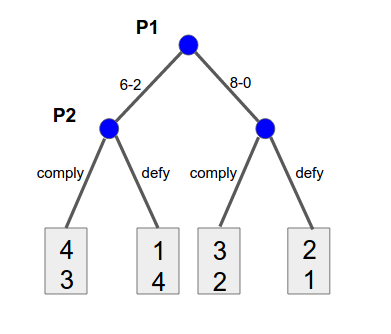
\includegraphics[width=1\columnwidth]{2_gt1.png}
\caption{Game Tree}


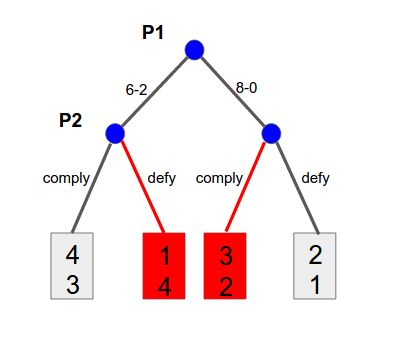
\includegraphics[width=1\columnwidth]{2_gt2.png}
\caption{Backward Induction: Player 2}
\label{2_gt2}


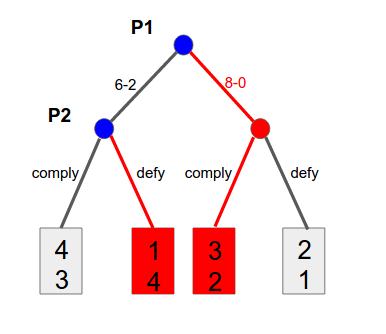
\includegraphics[width=1\columnwidth]{2_gt3.png}
\caption{Backward Induction: Player 1}
\label{2_gt3}
\end{multicols}
\end{figure}

By Backward Induction, \emph{Player 2 argues} that if the decision is \emph{6-2}, then it is better to \emph{defy}, since $4$ is better than $3$. If the decision, is \emph{8-0}, then it is better to \emph{comply}, since $2$ is better than $1$. This is illustrated in Figure \ref{2_gt2}. Now, \emph{Player 1 argues} that if the decision is \emph{6-2}, then Player 2 will \emph{defy} and the payoff is $1$. But, if the decision is \emph{8-0}, then Player 2 will comply and the payoff is $3$. Therefore, \emph{8-0} is better. \\ \\
Thus, the predicted outcome is \emph{\{ 8-0, comply \}}.

\section{Campus Shops}
\textbf{(a)} Let the price chosen by $S1$ be $p_1$, then if $S2$ choses $p_2$, the revenue generated by $S1$ and $S2$ is: 
$$\pi_{1} = p_1 \times (10-2p_1-p_2)$$
$$\pi_{2} = p_2 \times (10-p_1-2p_2)$$
Now, given $p_1$, $S2$ will choose $p_2$ such that $\pi_2$ is maximum, or:
$$\frac{\partial \pi_2}{\partial p_2}= 0$$
$$ 10 - p_1 -4p_2  = 0$$
$$p_2 = \frac{10-p_1}{4}$$
Now, since $S1$ knows the above strategy of $S2$, it will choose $p_1$, such that $\pi_1$ is maximum, given the above value of $p_2$:
$$\frac{\partial \pi_1}{\partial p_1}= 0$$
$$\frac{\partial}{\partial p_1}\Big(10p_1 - 2p_1^2 -p_1(\frac{10-p_1}{4})\Big)= 0$$
$$10 - 4p_1 - 10/4 + p_1/2 = 0$$
$$p_1 = 15/7 \sim 2.14$$
Therefore $p_2 = 55/28 \sim 1.96$. Thus, revenues are $\pi_1 = 8.03$ and $\pi_2 = 7.72$
\section{Tax Rate}
\section{Wireless Spectrum Block}
\section{Demonetised Note Auction}
\end{document}


